\documentclass[10pt,twocolumn]{article}

\usepackage[T1]{fontenc}
\usepackage[utf8]{inputenc}
\usepackage[margin=0.75in, top=1.0in, bottom=0.9in]{geometry}
\usepackage{newtxtext}
\usepackage{amsmath}
\usepackage{amssymb}
\usepackage{newtxmath}
\usepackage{microtype}
\usepackage[numbers,sort&compress]{natbib}
\usepackage[dvipsnames]{xcolor}
\usepackage[colorlinks=true, linkcolor=MidnightBlue, citecolor=MidnightBlue,
            urlcolor=MidnightBlue, bookmarks=false]{hyperref}
\usepackage{booktabs}
\usepackage{graphicx}
\usepackage{placeins}
\graphicspath{{../results/}}
\usepackage{algorithm}
\usepackage{algpseudocode}
\usepackage[small, labelfont=bf, font=small, skip=4pt]{caption}
\usepackage{titlesec}
\usepackage{enumitem}
\setlist{nosep, leftmargin=1.2em}

% ---------- column / paragraph spacing ----------
\setlength{\columnsep}{0.25in}
\setlength{\parindent}{1em}
\setlength{\parskip}{0pt}

% ---------- section headings (clean NeurIPS/ICML style) ----------
\titleformat{\section}
  {\normalfont\large\bfseries}
  {\thesection}{0.6em}{}
\titleformat{\subsection}
  {\normalfont\normalsize\bfseries}
  {\thesubsection}{0.5em}{}
\titleformat{\subsubsection}[runin]
  {\normalfont\normalsize\bfseries}
  {\thesubsubsection}{0.5em}{}[.\hspace{0.3em}]
\titlespacing*{\section}    {0pt}{10pt plus 2pt minus 1pt}{4pt}
\titlespacing*{\subsection} {0pt}{8pt plus 1pt}{3pt}

% ---------- clean page style (no header rules) ----------
\pagestyle{plain}

\begin{document}

\twocolumn[{%
\begin{center}
\vspace*{-0.3in}
  {\LARGE\bfseries When More Observation Hurts:\\[3pt]
  Redundancy and Robust Clarification\\[1pt]
  in Ask-or-Act Under Instruction Ambiguity}\\[12pt]
  {\large Zhu Yufan}\\[4pt]
  {\small National University of Singapore \quad\textbar\quad CS6208 Final Report}\\[2pt]
  {\small\texttt{A0238993J} \quad\textbar\quad April 10, 2026}
\end{center}
\vspace{12pt}
\centerline{\parbox{0.92\textwidth}{\small
\textbf{Abstract.}\enspace
In cooperative assistance an agent receives goal evidence through two channels: passive inference from observed actions and active clarification via costly questions.
In a controlled gridworld benchmark, we find that a cost-aware ask-or-act policy uses these channels \emph{sub-additively}: channel ablations reveal an interaction of $-26 \pm 3$\,pp at $K{=}3$, indicating overlapping rather than unique information extraction.
We further show that assistability is non-monotonic in principal rationality, as a \emph{more} rational principal can be harder to assist when action aliasing hides intent.
Under model mismatch, additional observation actively poisons the posterior, costing $-2.2$\,pp per step compared to $-0.8$ under matched conditions.
A surprise-tempered posterior update mitigates this by preserving matched performance while gaining $+1$--$+5$\,pp under mismatch, suggesting that posterior quality is at least as important as the ask-or-act policy under misspecification.
}}
\vspace{14pt}
}]

\section{Introduction}

A central challenge in cooperative assistance is deciding when a helper should ask for clarification rather than act.
Acting immediately risks committing to the wrong goal, whereas asking too often wastes time and may frustrate the principal.
The trade-off depends on the informativeness of available questions, the cost of a wrong action, and what the principal's behaviour already reveals.

We study this question by constructing an attribute-structured, post-parsing clarification benchmark in which the candidate goal set is known, question semantics are fixed, and the principal model is given.
The benchmark's value is controlled diagnosis, not ecological realism.
It includes a cooperative principal whose actions are observable for passive inference via inverse planning, and a question bank the assistant may use at explicit cost for active clarification.
The contributions are threefold, comprising a reproducible two-room gridworld with templated instruction ambiguity and a Boltzmann principal model, a systematic comparison of six ask-or-act policies across 19{,}800 episodes, and an empirical characterisation of how the two channels interact.
Our contribution is not a new ask policy, but, to our knowledge, the first controlled characterisation of how the value of active clarification changes as passive action evidence weakens, with the empirical success--question-cost frontier shifting substantially with principal rationality.

\textbf{Why a controlled benchmark?}
Prior work studies each channel in isolation. CLIPS~\cite{tan2024clips} performs inverse planning without asking, while ATD~\cite{kobalczyk2025active}, SAGE~\cite{suri2025structured}, and Grand et al.~\cite{grand2026shoot} study clarification without action-based inference.
To our knowledge, no prior benchmark combines both channels with controlled ambiguity sweeps (Table~\ref{tab:prior_work}).

\begin{table}[h]
\centering
\caption{Illustrative comparison to closest prior work (not an exhaustive survey).
\checkmark~=~present; $\circ$~=~partial; --~=~absent.}
\label{tab:prior_work}
\resizebox{\columnwidth}{!}{%
\small
\setlength{\tabcolsep}{4pt}
\begin{tabular}{lccccccc}
\toprule
Feature & \rotatebox{60}{CLIPS} & \rotatebox{60}{GRD} & \rotatebox{60}{PAGR} & \rotatebox{60}{ATD} & \rotatebox{60}{ShootFirst} & \rotatebox{60}{\textbf{Ours}} \\
\midrule
Action-based goal inference    & \checkmark & $\circ$ & \checkmark & -- & -- & \checkmark \\
Explicit ask-or-act decision   & -- & -- & $\circ$ & \checkmark & \checkmark & \checkmark \\
Typed questions with cost $c_q$& -- & -- & -- & \checkmark & -- & \checkmark \\
Task completion (not just recog.)& \checkmark & -- & -- & \checkmark & \checkmark & \checkmark \\
Controlled ambiguity-$K$ sweep & -- & -- & -- & -- & -- & \checkmark \\
Ground-truth task success      & $\circ$ & -- & -- & -- & $\circ$ & \checkmark \\
\bottomrule
\end{tabular}}
\end{table}

The gap is the ability to study how passive and active evidence \emph{interact}---substituting, complementing, or even conflicting---under a shared objective.

\textbf{Three Takeaways.}
\begin{enumerate}
  \item \textbf{Under AskOrAct, the two channels are used sub-additively.} Channel ablations show a negative interaction of $-26$\,pp at $K{=}3$: the policy extracts overlapping information from each channel. Clarification is most valuable as robustness insurance when passive inference is weak.
  \item \textbf{Assistability is non-monotonic in principal rationality.} At $K{=}3$, NeverAsk success peaks at intermediate $\beta$ and drops at high $\beta$ because extreme rationality collapses action diversity and hides intent.
  \item \textbf{Under model mismatch, more observation actively poisons the posterior.} Forced observation costs $-2.2$\,pp per step under mismatch compared to $-0.8$ under matched conditions, which is $2.8\times$ worse, explaining why passive-aware heuristics cannot outperform the simple cost-comparing baseline.
\end{enumerate}
Beyond the present comparison, the benchmark is intended as a reusable diagnostic testbed for future ask-or-act methods, enabling controlled evaluation as ambiguity, action informativeness, and question cost vary independently.

\section{Related Work}

\textbf{Goal inference and inverse planning.}
Inverse planning infers goals from behaviour~\cite{baker2009,ramirez2010plan}. CIRL~\cite{hadfield2016cirl} formalises cooperative teams with reward uncertainty, and CLIPS~\cite{tan2024clips} combines action and language evidence.
None provides an explicit ask-or-act decision.

\textbf{Shared autonomy and HRI clarification.}
Javdani et al.~\cite{javdani2015shared} blend assistance via hindsight optimisation, while Tellex et al.~\cite{tellex2014asking} and Cakmak and Thomaz~\cite{cakmak2012designing} study robot clarification questions.
Our setting decouples the principal and assistant and adds an explicit question cost.

\textbf{Goal recognition design and active sensing.}
GRD~\cite{keren2014grd} reduces shared action prefixes to improve legibility, Dragan et al.~\cite{dragan2013legibility} study legible motion, and Zhang et al.~\cite{zhang2025pagr} combine passive recognition with active information gathering in grids.
Our work differs in studying \emph{task completion} with typed costly questions and a shared success/cost objective.

\textbf{Ask-or-act under explicit cost.}
ATD~\cite{kobalczyk2025active} and SAGE~\cite{suri2025structured} frame LLM clarification as BED/EVPI, and Grand et al.~\cite{grand2026shoot} study ask-vs-act in language games.
None includes a cooperative principal whose actions are observed for inverse planning, precluding measurement of channel interaction.

\section{Method}

\subsection{Environment}

We use a $9{\times}9$ two-room gridworld with $M{=}6$ object instances per episode.
A vertical wall at the grid midpoint divides the space into \textit{Room~0} on the left and \textit{Room~1} on the right, connected by a single doorway at the central cell (Figure~\ref{fig:gridworld}).
Each episode samples 6 objects from the type set $\{\text{key}, \text{gem}, \text{coin}\}$ and colour set $\{\text{red}, \text{blue}, \text{green}\}$; exactly $K$ match the ambiguous instruction (candidate goals) and the remaining $M{-}K$ are distractors.

\begin{figure}[t]
  \centering
  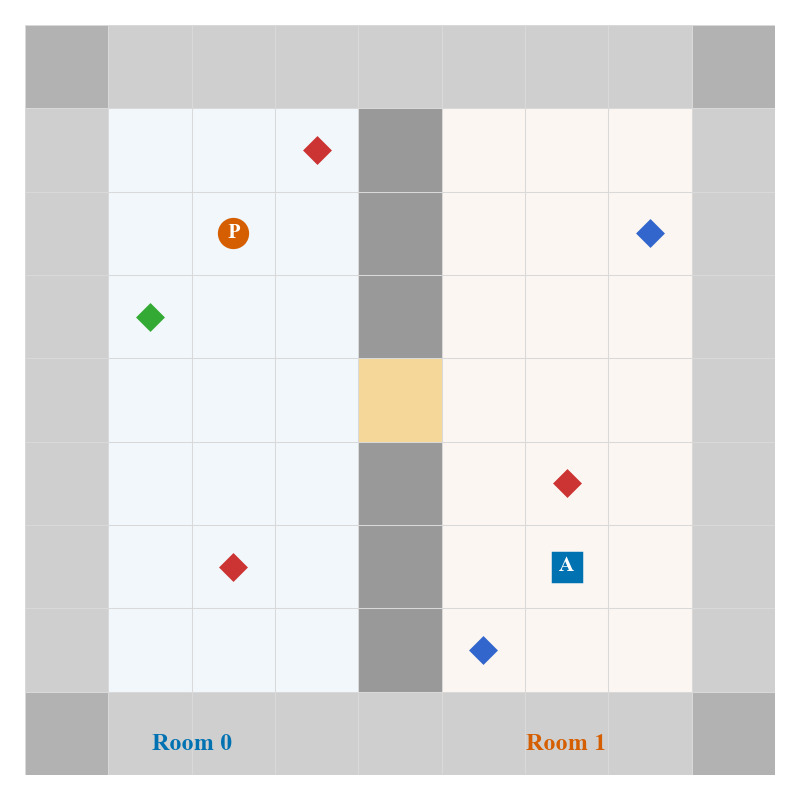
\includegraphics[width=\columnwidth]{gridworld_layout.png}
  \caption{Two-room $9{\times}9$ gridworld layout.  Room~0 (blue, left) and Room~1 (yellow, right) are separated by a wall with a single doorway.  Gold rings mark the $K{=}2$ candidate goals that match the instruction ``Bring me the red object''.  P~=~principal, A~=~assistant.}
  \label{fig:gridworld}
\end{figure}

A principal has a hidden goal object.
An instruction template maps the goal to a surface form shared by $K$ candidate goals (ambiguity level $K$).
The principal takes approximately rational actions towards its goal, sampled from a Boltzmann policy with rationality $\beta$ and $\varepsilon$-greedy noise:
$\pi_{\beta,\varepsilon}(a \mid s, g) = (1{-}\varepsilon)\,\mathrm{softmax}_\beta\bigl(V(s,\cdot,g)\bigr)_a + \varepsilon/|A|$,
where $V(s,a,g) = -d^*(\mathrm{succ}(s,a),\, g)$ is the negated shortest-path distance from the successor of $a$ to $g$.

The assistant observes the state, instruction, and all principal actions, but not the true goal.
An episode ends when the assistant picks an object, which counts as success if correct, or when the step budget $T_{\max}{=}200$ is exhausted.
The question bank $\mathcal{Q}$ contains three types of questions addressing the goal's colour, room, and object type, each with a factual answer drawn from a per-type noisy channel.
When the assistant decides to ask, it remains at its current position. When it decides to act, it takes one step toward the MAP-goal object via A* navigation and then re-evaluates.

\textbf{Running example.}
With ``bring me the red object'' ($K{=}3$), AskOrAct compares $\mathrm{CostAct}$ against $\mathrm{CostAsk}$, finds asking cheaper, and asks ``what type?''.
After receiving ``key'', the posterior concentrates and the agent acts.
InfoGainAsk asks more aggressively (entropy-gated, no cost comparison).
Table~\ref{tab:setup} summarises all hyperparameters.
Figure~\ref{fig:setup_overview} shows the full cooperative setup.

\begin{table}[h]
\centering
\caption{Environment and policy hyperparameters.}
\label{tab:setup}
\small
\begin{tabular}{ll}
\toprule
Parameter & Value \\
\midrule
Grid size & $9{\times}9$, two rooms \\
Objects & 6 (3 types $\times$ 3 colours) \\
Step budget $T_{\max}$ & 200 \\
Question bank $|\mathcal{Q}|$ & 3 (color, room, object) \\
Ask budget $Q_{\max}$ & 3 \\
Ask window & steps $\leq 6$ \\
Question cost $c_q$ & 0.5 \\
Entropy gate $\tau_H$ (AskOrAct) & 0.3 \\
IG threshold $\tau_{\mathrm{IG}}$ & 0.01 \\
Answer noise (color/room/object) & 0.05 / 0.10 / 0.20 \\
Principal rationality $\beta$ & 2.0 (default) \\
Principal noise $\varepsilon$ & 0.05 (default) \\
\bottomrule
\end{tabular}
\end{table}

\begin{figure}[t]
  \centering
  
\includegraphics[width=\columnwidth]{setup_overview.png}
  \caption{Task setup. The principal has a hidden goal in a two-room gridworld; the assistant sees the world state, an ambiguous instruction, and the principal's movement. Questions can collapse the posterior over candidate goals.}
  \label{fig:setup_overview}
\end{figure}

\subsection{Bayesian Posterior}

\textbf{Per-step protocol.}
At each step the assistant first observes the principal's action, then updates $b_t$ from the action, then chooses whether to ask or act. If asking, it receives an answer and updates $b_t$. If acting, it moves one step via A* toward the MAP goal. This cycle then repeats.

The assistant maintains a posterior $b_t(g)$ over candidate goals $\mathcal{G}$.
Initialisation uses the instruction likelihood under each goal.
After observing principal action $a_t$ at state $s_t$:
\[
  b_{t+1}(g) \propto b_t(g) \cdot \pi_{\hat\beta,\hat\varepsilon}(a_t \mid s_t, g),
\]
where $\hat\beta, \hat\varepsilon$ are the assistant's assumed principal parameters, matched to the true values unless otherwise noted in the mismatch analysis.

When a question $q$ is asked and answered $\alpha$, the posterior is updated by the answer likelihood:
\[
  b(g) \propto b(g) \cdot P(\alpha \mid q, g, \text{noise}),
\]
where the answer noise varies by type, with color at 0.05, room at 0.10, and object at 0.20.

\subsection{Ask-or-Act Policy}

\textit{AskOrAct} uses a Bayes-risk ask gate to decide \emph{whether} to ask, paired with a separate MAP$+$A* controller for motion execution.
The ask gate compares the expected surrogate team cost, defined as navigation steps plus per-question penalty $c_q$, of asking versus acting under the current posterior $b_t$.
The policy is not a unified Bayes-risk controller since the ask decision uses expected cost while the act branch greedily follows A* toward the MAP goal.
It serves as an analytically computable reference for locating one operating point on the empirical success--question-cost frontier, not as a proposed optimal policy.

Formally, at step $t$, the assistant computes:
\[
  \text{CostAct} = \sum_{g} b_t(g) \cdot d^*(s_t, g),
\]
the expected obstacle-aware shortest-path distance computed via A* to each candidate goal under the current posterior, and
\[
  \text{CostAsk}(q) = \underbrace{1}_{\text{step}} + \underbrace{c_q}_{\text{question}} + \mathbb{E}_{\alpha}\bigl[\text{CostAct}(b_{t,q,\alpha})\bigr],
\]
where asking incurs both one timestep of delay costing $1$ and an additional penalty $c_q = 0.5$ for the principal's effort, and the expectation integrates over answers $\alpha$ after updating to $b_{t,q,\alpha}$.
This one-step myopic lookahead does not plan over multi-step ask sequences.

\textbf{Decision rule.}
The policy selects $\arg\min_q \text{CostAsk}(q)$ when $\min_q \text{CostAsk}(q) < \text{CostAct}$, and acts otherwise.
Because the surrogate cost $C$ does not penalise wrong picks, this comparison minimises effort under the current posterior but does not account for failure risk.

\textbf{Heuristic guards.}
Three heuristic constraints are imposed on top of the Bayes-risk core for engineering robustness and are not part of the decision-theoretic derivation.
\begin{enumerate}
  \item \textbf{Entropy gate.} The ask branch is skipped when $H(b_t) \leq 0.3$, providing a fast exit when the posterior is already concentrated. This guard is technically redundant with CostAsk but avoids floating-point edge cases.
  \item \textbf{Ask window.} Questions are disallowed after step 6, preventing late questions that cannot pay off before the step deadline.
  \item \textbf{Budget.} At most $Q_{\max} = 3$ questions per episode, matching the 3 available question types.
\end{enumerate}
All thresholds, including $\tau_H$, $\tau_\mathrm{IG}$, the ask window, and $Q_\mathrm{max}$, are hand-set rather than tuned on a validation split. The ablation in Section~\ref{sec:results} shows that $c_q$ dominates and performance is insensitive to the guard parameters within reasonable ranges, as detailed in Appendix~\ref{app:hyperparams}.
Figure~\ref{fig:ask_or_act_pipeline} summarises this decision process from instruction grounding through posterior update and the final ask-versus-act comparison.

\subsection{Surprise-Tempered Updates (AskOrAct-ST)}

Under model mismatch, standard Bayesian updates can poison the posterior as shown in Section~\ref{sec:results}.
We address this with a surprise-triggered likelihood tempering that modifies the passive update without changing the ask-or-act policy:
\[
  b_{t+1}(g) \propto b_t(g) \cdot \pi(a_t \mid s_t, g, \hat\beta)^{\omega_t},
\]
where $\omega_t \in (0, 1]$ controls how much the passive observation is trusted.
The tempering weight is driven by a CUSUM-style surprise accumulator:
\[
  S_t = \max\bigl(0,\; \gamma\, S_{t-1} + \bigl(-\!\log p_t(a_t) - \mu\bigr)\bigr),
  \quad \omega_t = \frac{1}{1 + S_t / \tau},
\]
where $p_t(a_t) = \sum_g b_t(g)\,\pi(a_t \mid s_t, g, \hat\beta)$ is the predictive action probability, $\mu{=}1.5$ is the matched-model baseline surprise, $\gamma{=}0.9$ is the forgetting rate, and $\tau{=}3.0$ is the tempering scale.
Under a matched model, $S_t \approx 0$ so $\omega_t \approx 1$, recovering standard Bayesian updating.
Under mismatch, $S_t$ grows and $\omega_t$ shrinks, downweighting unreliable passive evidence.

This intervenes at the \emph{inference} layer rather than the decision layer, and the ask-or-act gate remains unchanged.
Three prior attempts to improve the decision layer all failed as described in Section~\ref{sec:results}, motivating an inference-layer intervention instead.

\subsection{Baselines}

Let $\mathcal{Q}$ denote the question bank, $Q_{\max}{=}3$ the per-episode ask budget, $\tau_H$ the entropy gate set to $0.3$ for AskOrAct and $0.5$ for baselines, and $\tau_{\mathrm{IG}}{=}0.01$ the information-gain threshold. A matched-gate check with $\tau_H{=}0.3$ for all policies preserves the ordering.
Define the information gain of question $q$ under belief $b_t$ as:
\[
  \mathrm{IG}(q, b_t) = H(b_t) - \sum_{\alpha} P(\alpha \mid q, b_t)\, H(b_{t,q,\alpha}),
\]
where $b_{t,q,\alpha} \propto b_t(g)\cdot P(\alpha \mid q, g)$ is the posterior after observing answer $\alpha$.

\textbf{NeverAsk} always acts toward the MAP goal and never asks.

\textbf{AlwaysAsk} asks $q^*{=}\arg\max_{q \in \mathcal{Q}} \mathrm{IG}(q,b_t)$ whenever permitted by the shared entropy and budget gates, specifically $H(b_t)>\tau_H$ and $|\text{asked}|<Q_{\max}$, and otherwise acts toward MAP.

\textbf{InfoGainAsk} uses the same gating as AlwaysAsk but additionally requires $\mathrm{IG}(q^*,b_t)>\tau_{\mathrm{IG}}$.
Let $C_{\mathrm{IG}} \equiv |\text{asked}|<Q_{\max} \wedge H(b_t)>\tau_H \wedge \mathrm{IG}(q^*,b_t)>\tau_{\mathrm{IG}}$. Then
\[
  \pi_{\mathrm{IG}}(b_t) =
  \begin{cases}
    \mathrm{ask}(q^*) & \text{if } C_{\mathrm{IG}} \\
    \mathrm{act}(\arg\max_g b_t(g)) & \text{otherwise.}
  \end{cases}
\]

\textbf{EasyInfoGainAsk} is identical to InfoGainAsk but uses budget $Q_{\max}^{\mathrm{easy}}{=}1$ and no entropy gate.
Let $C_{\mathrm{EIG}} \equiv |\text{asked}|<1 \wedge \mathrm{IG}(q^*,b_t)>\tau_{\mathrm{IG}}$. Then
\[
  \pi_{\mathrm{EIG}}(b_t) =
  \begin{cases}
    \mathrm{ask}(q^*) & \text{if } C_{\mathrm{EIG}} \\
    \mathrm{act}(\arg\max_g b_t(g)) & \text{otherwise.}
  \end{cases}
\]

\textbf{RandomAsk} uses the same ask-gating condition as InfoGainAsk but selects a question uniformly at random from unanswered questions.

\textbf{POMCPPlanner} is a limited sanity-check baseline using POMCP~\cite{silver2010pomcp} tree search with 250 iterations and horizon 8. It probes whether a budget-limited online planner can match analytical policies in this small environment and should not be read as representative of the best achievable planning performance.

\textbf{EasyInfoGainAsk} and \textbf{POMCPPlanner} are side diagnostics evaluated only at $K{=}2$, the most competitive setting for asking, and are not part of the main comparison across $K$.

\section{Experimental Setup}
\label{sec:setup}

\textbf{Sweep.}
The main evaluation covers $K \in \{1,2,3,4\}$, $\varepsilon \in \{0, 0.05, 0.1\}$, $\beta \in \{1, 2, 4\}$, 5 replicate seeds $\times$ 20 episodes per condition = 100 episodes per cell.
The 5 core policies are evaluated in every cell, and \textit{EasyInfoGainAsk} and \textit{POMCPPlanner} are additionally evaluated at $K{=}2$.
This yields a total of 19{,}800 episodes.

\textbf{Metrics.}
The two primary axes are \textit{success rate}, the fraction of episodes where the assistant picks the true goal, and \textit{questions asked}, averaged per episode.
Together these define the empirical success--question-cost frontier.
We also report the \textit{surrogate team cost} $C {=} \text{steps} {+} c_q {\cdot} |\text{questions}|$, the effort scalar AskOrAct minimises. Note that $C$ does not penalise wrong picks, as success rate captures that dimension.
\textit{Regret} $= C - C^*_{\text{oracle}}$ measures excess effort relative to the oracle's shortest-path cost $C^*_{\text{oracle}}$.
Because $C$ does not penalise wrong picks, regret is a secondary diagnostic and success rate is the primary outcome.

\textbf{Statistics.}
Each condition pools 100 episodes drawn from 5 seeds with 20 episodes per seed.
For the key comparative claims, we report \textit{paired seed-level deltas}, defined as the per-seed success difference between policies averaged over the 5 seeds with $\pm$1 s.e.\ across seeds.
95\% bootstrap CIs with $B{=}1000$ episode-level resamples are shown in figures as a secondary measure of within-condition variability.
Full per-$(K,\varepsilon,\beta)$ breakdowns appear in Appendix~B.

\begin{figure}[t]
  \centering
  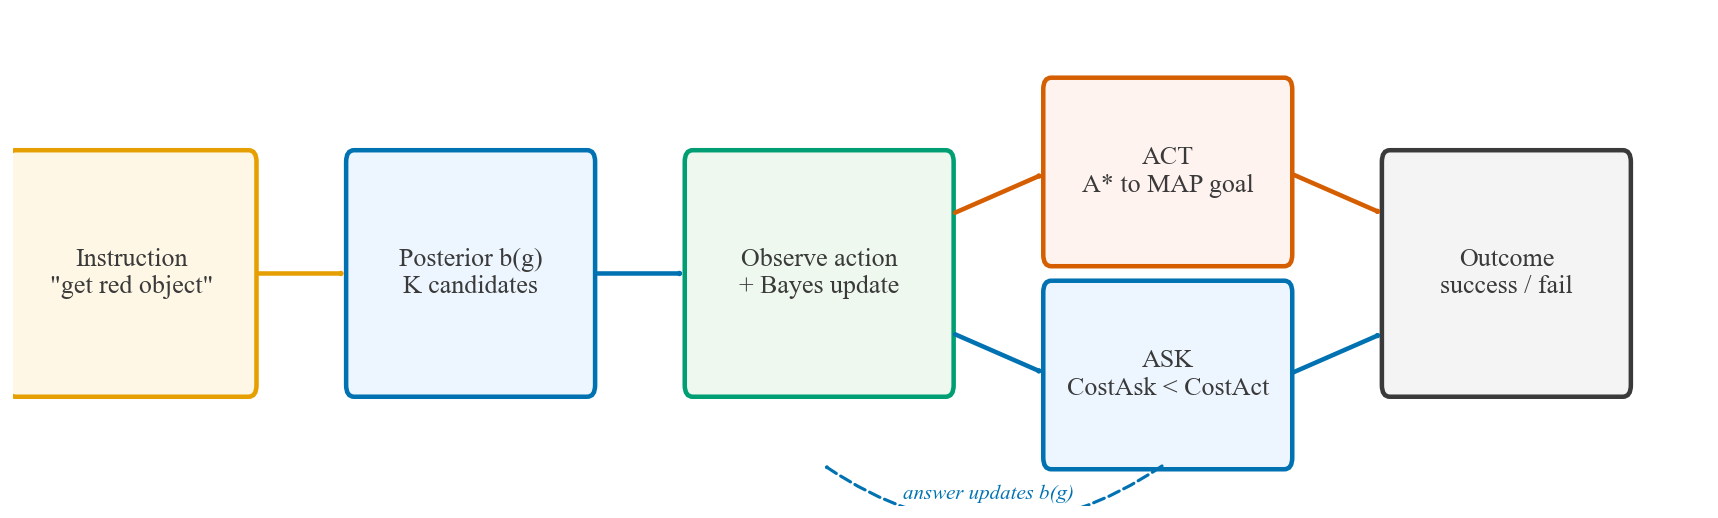
\includegraphics[width=\columnwidth]{ask_or_act_pipeline.png}
  \caption{AskOrAct decision flow: instruction $\to$ posterior $\to$ observe + update $\to$ ASK or ACT. Dashed: answer feeds back.}
  \label{fig:ask_or_act_pipeline}
\end{figure}

\section{Results}
\label{sec:results}

\subsection{Main Sweep}

\begin{figure}[t]
  \centering
  
\includegraphics[width=\columnwidth]{main_dashboard.png}
  \caption{Success rate, regret, and questions asked by ambiguity $K$ (averaged over $\varepsilon$, $\beta$; error bars: 95\% bootstrap CI). Policies diverge at $K{\geq}3$; InfoGainAsk trades more questions for higher success.}
  \label{fig:main}
\end{figure}

Figure~\ref{fig:main} shows results averaged across all $\varepsilon$ and $\beta$ conditions.
At $K{=}1$, where there is no ambiguity, all policies perform identically with 100\% success and zero questions.
As ambiguity rises to $K{\geq}3$, policies diverge.

\textbf{Caveat: K is not a pure manipulation.}
Template feasibility changes with $K$. For example, $T1$ is used only at $K{=}1$ and $T2$ is excluded at $K{\geq}2$.
Table~\ref{tab:t3} isolates the ambiguity effect by restricting to the color-only template T3 across $K{\in}\{2,3,4\}$ with 500 episodes per cell.
AskOrAct--NeverAsk deltas are $-2$, $+3$, and $+7$\,pp, confirming the advantage grows with $K$ within a single template family.

\begin{table}[h]
\centering
\caption{Within-template T3 (color-only). Isolates the effect of $K$.}
\label{tab:t3}
\scriptsize
\begin{tabular}{llrr}
\toprule
$K$ & Policy & Success & Q/ep \\
\midrule
2 & AskOrAct & 95\% & 0.61 \\
  & NeverAsk & 97\% & 0.00 \\
\midrule
3 & AskOrAct & 90\% & 0.67 \\
  & NeverAsk & 87\% & 0.00 \\
\midrule
4 & AskOrAct & 92\% & 0.61 \\
  & NeverAsk & 85\% & 0.00 \\
\bottomrule
\end{tabular}
\end{table}

Table~\ref{tab:main} summarises the key aggregate results, and full per-$(K,\varepsilon,\beta)$ results appear in Appendix~B.

\begin{table}[h]
\centering
\caption{Mean results averaged over all $(\varepsilon, \beta)$ conditions. $C$ = surrogate team cost (steps $+ c_q {\cdot}$ questions; lower is better). \textbf{Bold}: best success; \underline{uline}: lowest $C$ (secondary).}
\label{tab:main}
\small
\begin{tabular}{llrrrr}
\toprule
$K$ & Policy & Success & $C\!\downarrow$ & Regret & Q/ep \\
\midrule
2 & InfoGainAsk & \textbf{96.9\%} & 8.78 & 2.25 & 1.05 \\
  & AskOrAct           & 96.7\%          & \underline{8.04} & 1.71 & 0.65 \\
  & AlwaysAsk          & 94.6\%          & 10.31 & 3.44 & 1.87 \\
  & NeverAsk           & 91.1\%          & 8.20 & 1.67 & 0.00 \\
\midrule
3 & InfoGainAsk & \textbf{94.8\%} & 9.82 & 2.61 & 1.21 \\
  & AskOrAct           & 91.7\%          & \underline{8.81} & 2.14 & 0.67 \\
  & AlwaysAsk          & 90.2\%          & 11.87 & 4.08 & 2.29 \\
  & NeverAsk           & 83.8\%          & 9.23 & 2.15 & 0.00 \\
\midrule
4 & InfoGainAsk & \textbf{91.7\%} & 10.54 & 2.88 & 1.31 \\
  & AskOrAct           & 87.3\%          & \underline{9.43} & 2.42 & 0.61 \\
  & AlwaysAsk          & 86.4\%          & 13.08 & 4.56 & 2.58 \\
  & NeverAsk           & 78.9\%          & 9.88 & 2.40 & 0.00 \\
\bottomrule
\end{tabular}
\end{table}

\textbf{The frontier: InfoGainAsk vs.\ AskOrAct.}
\textit{InfoGainAsk} attains $+3.1$--$+4.4$\,pp higher success at $K{=}3,4$ using ${\sim}2\times$ more questions.
AskOrAct achieves the lowest surrogate cost $C$ at every $K$, and neither policy is universally preferable without an application-specific exchange rate.

\textbf{Gain from asking: AskOrAct vs.\ NeverAsk.}
At $K{=}3$ the gain is $+7.9 \pm 1.2$\,pp, with mean $\pm$ s.e.\ over 5 seeds and a 95\% CI of $[5.0, 10.8]$.
At $K{=}4$ the gain is $+8.4 \pm 1.4$\,pp with a 95\% CI of $[5.1, 12.1]$.
The effect is positive for every seed with only $0.61$--$0.67$ questions per episode.
\textit{AlwaysAsk} asks $2.3$--$2.6\times$ more but achieves lower or similar success, confirming over-asking is costly.

\subsection{Robustness}

\textbf{Answer noise (exploratory).}
An independently-sampled sweep varies answer noise from 0 to 0.2. Because episodes are not seed-matched across levels, this analysis is exploratory as detailed in Appendix~\ref{app:robustness}.

\textbf{$\beta$-mismatch.}
With $\hat\beta{=}2$ fixed and true $\beta{\in}\{1,2,4\}$, the hardest case of $\beta{=}1$ with a near-random principal still yields $+13.5$\,pp for AskOrAct over NeverAsk.

\textbf{Scale-$K$.}
Extending to $K \in \{5, 6\}$ shows that the asking advantage grows. \textit{AskOrAct} retains meaningful success while \textit{NeverAsk} falls substantially, consistent with VoI being most valuable under high ambiguity.

\textbf{Non-monotonic assistability in principal rationality.}
Figure~\ref{fig:beta_u} sweeps $\beta$ from 0.5 to 16 with matched models.
At $K{=}3$, NeverAsk success peaks at $\beta{=}8$ with $92\%$ and then \emph{drops} to $84\%$ at $\beta{=}16$ because extreme rationality collapses action diversity among aliased goals, hiding the principal's intent.
AskOrAct detects this and responds by increasing its Q/ep from 0.52 at $\beta{=}8$ to 0.60 at $\beta{=}16$, maintaining $92\%$.
At $K{=}4$ the effect is weaker, and we report it as regime-dependent rather than universal.

\begin{figure}[t]
  \centering
  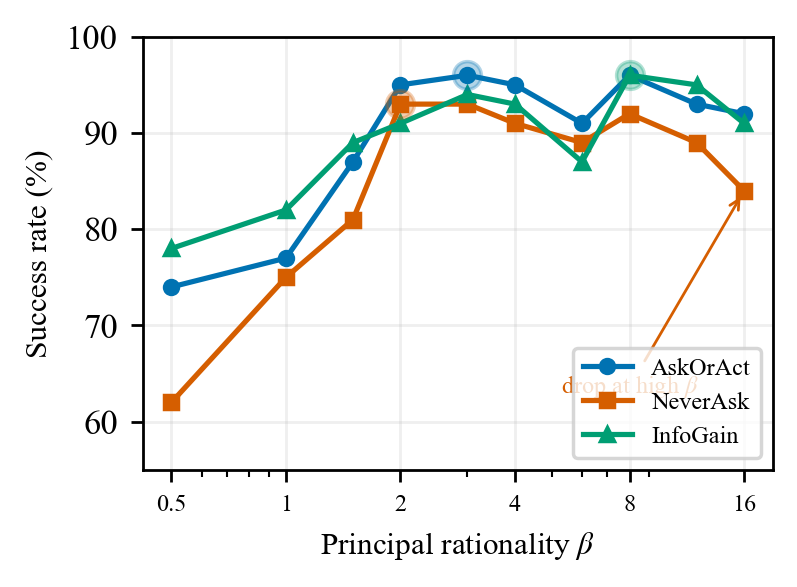
\includegraphics[width=\columnwidth]{beta_inverted_u.png}
  \caption{Success vs.\ $\beta$ at $K{=}3$. NeverAsk drops at high $\beta$ (action aliasing); AskOrAct compensates. $K{=}4$ shows a weaker effect (not shown).}
  \label{fig:beta_u}
\end{figure}

\textbf{Path overlap determines ask-worthiness.}
Define \emph{overlap} $= |\{g \in \mathcal{G} : a^*(g) = \text{mode}\}| / K$, the fraction of candidates sharing the modal optimal first action from the principal's position.
Table~\ref{tab:overlap} stratifies $K{=}3$ episodes by this metric.
When goals diverge (overlap ${<}0.5$), NeverAsk matches AskOrAct at $100\%$.
When fully aliased (overlap ${=}1.0$), NeverAsk collapses to $64.5\%$ while AskOrAct maintains $87.1\%$ ($+22.6$\,pp).
The ``diverge'' bucket is small with only $n{=}7$ episodes, and the analysis is limited to $K{=}3$, so the pattern is suggestive rather than definitive.

\begin{table}[h]
\centering
\caption{Path overlap vs.\ success at $K{=}3$.}
\label{tab:overlap}
\scriptsize
\begin{tabular}{lrrrr}
\toprule
Overlap & AskOrAct & NeverAsk & $\Delta$ & $n$ \\
\midrule
Diverge ($<$0.5)  & 100.0\% & 100.0\% & $0$ & 7 \\
Partial (0.5--0.99) & 95.2\% & 98.4\% & $-3.2$ & 62 \\
Aliased (1.0)     & 87.1\% & 64.5\% & $+22.6$ & 31 \\
\bottomrule
\end{tabular}
\end{table}

\textbf{More observation can hurt under mismatch.}
Figure~\ref{fig:obs_hurts} forces $h$ observation steps before allowing any ask/act decision at $K{=}4$.
Under matched models, success declines gently from $88\%$ to $84\%$, a drop of $-4$\,pp over 5 steps.
Under mismatch with $\beta_\text{true}{=}1$ and $\hat\beta{=}2$, the same forced observation costs $-11$\,pp as success drops from $87\%$ to $76\%$, because the agent builds confidence in the wrong goal from mismodelled actions.
The slope difference of $-11$ versus $-4$\,pp confirms that passive inference is not merely less useful under mismatch but is actively harmful.

\begin{figure}[t]
  \centering
  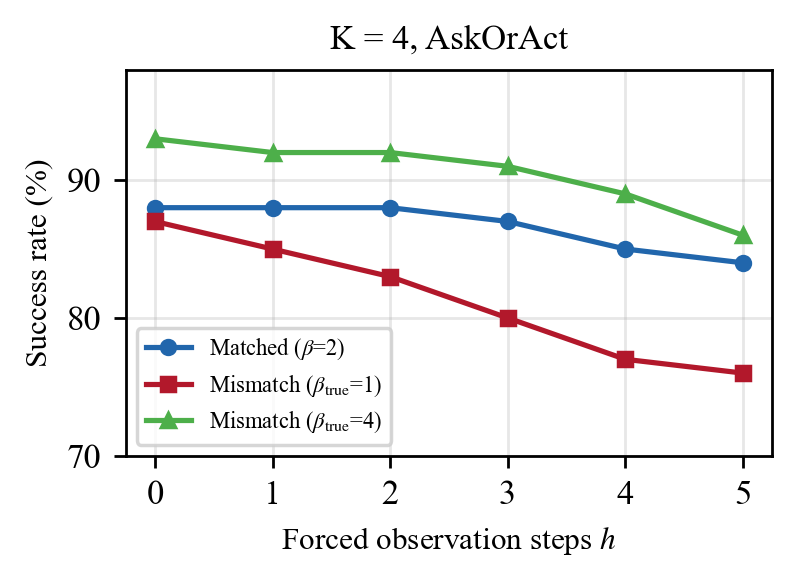
\includegraphics[width=\columnwidth]{obs_hurts_mismatch.png}
  \caption{Forced observation horizon $h$ vs.\ success at $K{=}4$. Under mismatch ($\beta_\text{true}{=}1$), more observation actively hurts.}
  \label{fig:obs_hurts}
\end{figure}

\textbf{Surprise-tempered updates mitigate mismatch.}
AskOrAct-ST as described in Section~3.4 addresses posterior poisoning by downweighting passive evidence when action surprise is high.
Table~\ref{tab:temper} shows paired seed-level deltas reported as mean $\pm$ 1\,s.e.\ over 5 seeds. There is no harm under matched models, with $+0.0 \pm 1.6$\,pp at $K{=}3$, and positive gains appear under mismatch. The largest gain of $+5.0 \pm 2.7$\,pp occurs at $\beta_\text{true}{=}0.5$ and $K{=}4$.
The gains are modest and some CIs include zero, so we characterise AskOrAct-ST as a \emph{mitigation} rather than a complete fix.
A sensitivity sweep over $\gamma{\in}\{0.7, 0.9, 0.95\}$ and $\tau{\in}\{1.5, 3.0, 6.0\}$ at the hardest condition of $K{=}4$ and $\beta{=}0.5$ shows all 9 settings improve by $+1$ to $+4$\,pp.

\begin{table}[h]
\centering
\caption{AskOrAct vs.\ AskOrAct-ST (surprise-tempered). $\Delta$: gain from tempering.}
\label{tab:temper}
\scriptsize
\begin{tabular}{llrrl}
\toprule
$K$ & Condition & AskOrAct & ST & $\Delta$ (pp) \\
\midrule
3 & Matched ($\beta{=}2$) & 95\% & 95\% & $+0.0 \pm 1.6$ \\
3 & Mismatch ($\beta{=}1$) & 78\% & 81\% & $+3.0 \pm 2.5$ \\
3 & Mismatch ($\beta{=}0.5$) & 73\% & 76\% & $+3.0 \pm 2.0$ \\
\midrule
4 & Matched ($\beta{=}2$) & 82\% & 82\% & $+0.0 \pm 0.0$ \\
4 & Mismatch ($\beta{=}1$) & 71\% & 72\% & $+1.0 \pm 1.9$ \\
4 & Mismatch ($\beta{=}0.5$) & 54\% & 59\% & $+5.0 \pm 2.7$ \\
\bottomrule
\end{tabular}
\end{table}

Three prior attempts to improve the \emph{decision layer}, namely the overlap heuristic, one-step lookahead, and surprise-triggered asking, all failed to beat AskOrAct by $-1$ to $-5$\,pp.
This suggests that under mismatch the posterior quality is at least as important as the ask-or-act gate, though the policy's surrogate objective, which ignores failure cost, may also contribute.

\textbf{Generalization.}
Layout, prior, noise, grid-size, and room-count variations all preserve a positive AskOrAct--NeverAsk gap of $+2$--$+8$\,pp at $K{=}4$, with details provided in Appendix~\ref{app:robustness}.

\textbf{Passive channel degradation.}
Figure~\ref{fig:action_drop} varies the fraction $p_\text{drop}$ of principal actions the assistant fails to observe.
As the passive channel weakens, AskOrAct increases its question rate from 0.66 to 1.11 Q/ep at $K{=}4$, and its paired seed-level advantage over NeverAsk grows from $+4.0 \pm 5.3$\,pp at $p_\text{drop}{=}0$ to $+23.0 \pm 3.4$\,pp at $p_\text{drop}{=}1$.
InfoGainAsk maintains a fixed ${\sim}1.5$ Q/ep regardless of $p_\text{drop}$, confirming that only the cost-aware policy adapts to passive channel quality.

\begin{figure}[t]
  \centering
  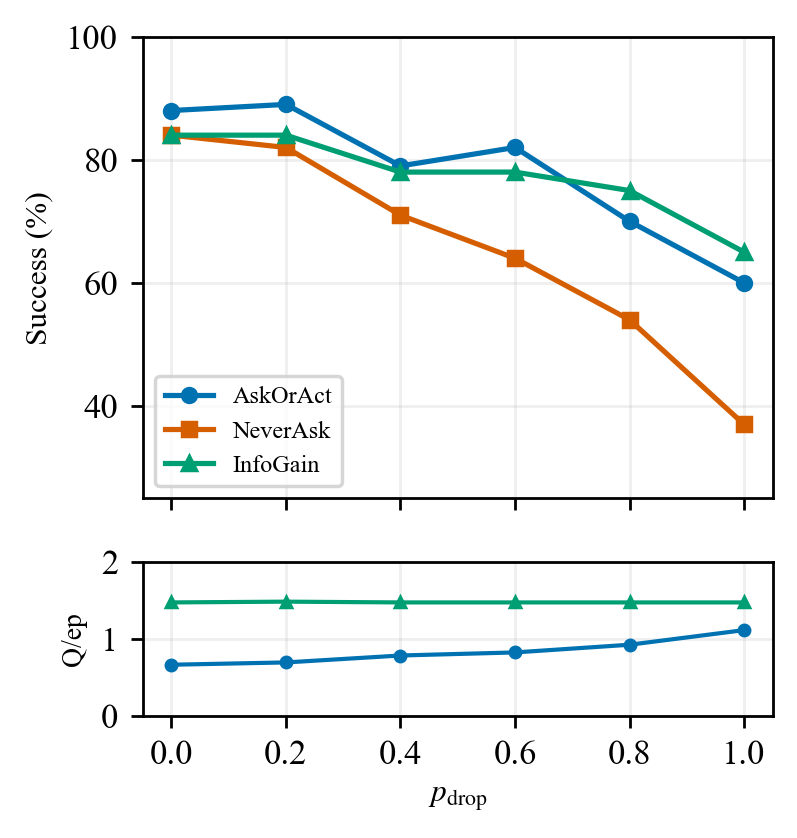
\includegraphics[width=\columnwidth]{action_drop_sweep.png}
  \caption{Passive channel degradation at $K{=}4$. Top: success rate vs.\ $p_\text{drop}$. Bottom: Q/ep. AskOrAct adaptively asks more as passive inference weakens.}
  \label{fig:action_drop}
\end{figure}

\textbf{Sub-additive channel use.}
We ablate AskOrAct's channels: \emph{both} (default), \emph{passive-only} ($Q_\text{max}{=}0$), \emph{active-only} ($p_\text{drop}{=}1$), \emph{neither} ($Q_\text{max}{=}0$, $p_\text{drop}{=}1$).
The interaction $I = V(\text{both}) - V(\text{passive}) - V(\text{active}) + V(\text{neither})$ is $-26 \pm 3.3$\,pp at $K{=}3$ and $-20 \pm 3.2$\,pp at $K{=}4$ (mean $\pm$ 1\,s.e.).
AskOrAct uses the channels sub-additively, extracting overlapping information; whether the channels are intrinsically redundant would require coalition-specific policy optimisation.
Clarification is most valuable when passive inference is weak or unreliable.

\begin{figure}[t]
  \centering
  
\includegraphics[width=\columnwidth]{synergy_decomposition.png}
  \caption{Channel ablation interaction under AskOrAct. Negative = sub-additive channel use. $I$ values annotated per $K$.}
  \label{fig:synergy}
\end{figure}



\subsection{Ablations}

\begin{table}[h]
\centering
\caption{Ablation results for \textit{AskOrAct} at $K{=}3,4$, averaged over $(\varepsilon, \beta)$ and ablation variants (wrong-pick-fail $\in\{$T,F$\}$, deadline margin $\in\{3,5,7\}$). Lower success than Table~\ref{tab:main} reflects the harsh variant mix.}
\label{tab:ablations}
\small
\begin{tabular}{llrrr}
\toprule
Mode & $c_q$ & Ask-step & Success & Q/ep \\
\midrule
A & 0.0 & yes & 69.2\% & 1.61 \\
B & 0.5 & no  & 73.6\% & 0.64 \\
C & 0.5 & yes & 73.8\% & 0.65 \\
\bottomrule
\end{tabular}
\end{table}

Table~\ref{tab:ablations} averages over ablation variants including wrong-pick termination (episode ends on wrong pick vs.\ continues) and deadline margins ($\pm2$ steps around optimal).
Mode~A with $c_q{=}0$ over-asks at 1.61 q/ep and degrades success, while Modes~B and~C show that the step-counting convention has negligible effect once $c_q{>}0$.
Non-zero question cost is the primary driver of selective asking.

\textbf{Clarification quality.}
AskOrAct's first question reduces posterior entropy by a similar amount to InfoGainAsk at $K{=}3,4$, while asking less often (details in Appendix).

\section{Discussion}

\textbf{Sub-additive channel use.}
Channel ablations of AskOrAct show a negative interaction ($I{=}-26 \pm 3$\,pp at $K{=}3$), indicating the policy extracts overlapping information from the two channels.
Asking matters most when passive inference is structurally unable to resolve ambiguity, as shown by the $+22.6$\,pp gain in the aliased regime.

\textbf{Surrogate vs.\ failure-aware cost.}
AskOrAct optimises surrogate cost $C$ without penalising wrong picks, yet when we post-hoc compute $C_f = C + c_\text{fail} \cdot \mathbf{1}[\text{fail}]$, AskOrAct achieves lower $C_f$ than NeverAsk for $c_\text{fail} \geq 10$, for instance $9.4$ versus $10.2$ at $K{=}3$ with $c_\text{fail}{=}10$.
The surrogate is thus a reasonable proxy for moderate failure penalties, though InfoGainAsk achieves even lower $C_f$ at higher question cost.

\textbf{The $\beta$ inverted-U and its mechanism.}
The non-monotonic assistability finding shown in Figure~\ref{fig:beta_u} follows from a proposition about first-action informativeness.

\textit{Observation.} Aliasing kills informativeness at high $\beta$.
Let $a^*(g)$ denote the optimal first action for goal $g$.
If $a^*(g) = a^*$ for all $g \in \mathcal{G}$ (first-action aliasing), then $I(\text{goal};\, a_1) \to 0$ as $\beta \to \infty$.

\textit{Proof sketch.}
Under the Boltzmann policy, as $\beta \to \infty$ the action distribution concentrates on the shared optimal action $a^*$ regardless of the true goal $g$, so $P(a \mid g) \to \mathbf{1}[a = a^*]$ for all $g$.
The marginal $P(a)$ equals $P(a \mid g)$ in this limit, giving $I = 0$.
At finite $\beta$, sub-optimal actions may still carry residual goal information, but this can decrease with $\beta$ in the aliased case---contrary to the intuition that ``more rational = more informative.''

Increasing $\beta$ therefore narrows the action distribution without increasing discriminative power, while reducing diversity that could accidentally reveal intent.
AskOrAct detects this regime and compensates by asking more.
This interaction requires both channels and is invisible in single-channel benchmarks~\cite{kobalczyk2025active,grand2026shoot,tan2024clips} and in recognition-only settings~\cite{keren2014grd,zhang2025pagr}.

\textbf{Passive inference as a double-edged sword.}
Under model mismatch, each forced observation step costs $-2.2$\,pp, which is $2.8\times$ the matched rate, actively poisoning the posterior as shown in Figure~\ref{fig:obs_hurts}.
Straightforward passive-aware heuristics such as overlap checks and one-step lookahead fail to improve over AskOrAct because the myopic cost comparison already internalises much of the passive information value.
An optimal policy should gate not only \emph{whether} to ask, but \emph{when} to stop trusting passive evidence---a design consideration absent from current ask-or-act methods.

\textbf{POMCP sanity check.}
Our budget-limited POMCP with 250 rollouts and horizon 8 underperforms analytical policies due to high branching factor and tree rebuilds. With more iterations and persistent trees it would be the appropriate baseline in larger state spaces.

\textbf{Limitations and Future Work.}
The question bank is fixed at three types, and extending to open-ended questions requires a generative answer model.
The gridworld is small enough for exact posteriors, and scaling to larger environments would require particle-filter or amortised inference.
The principal follows a Boltzmann model, whereas real principals may be non-stationary.
The $\beta$ inverted-U and observation-hurts findings are regime-dependent, observed at $K{=}3$ and under specific mismatch conditions, and the quantitative thresholds are benchmark-specific.
Future work could investigate failure-aware objectives since the myopic surrogate does not price wrong picks, as well as adaptive $c_q$ and richer environment structure.

\section{Conclusion}

We presented a controlled benchmark for ask-or-act decisions with both a diagnostic and a constructive contribution.
On the diagnostic side, AskOrAct uses the two channels sub-additively ($I{=}-26$\,pp), assistability is non-monotonic in principal rationality, and under mismatch observation actively poisons the posterior at $-2.2$\,pp per step.
On the constructive side, surprise-tempered posterior updates in AskOrAct-ST mitigate mismatch with no harm when matched and $+1$--$+5$\,pp gains under mismatch, after three decision-layer interventions all failed.
This suggests posterior quality is at least as important as the ask-or-act policy under misspecification.
As a scope note, these findings characterise behaviour in a controlled gridworld under a Boltzmann principal, and generalization to richer environments and real human principals remains an open question.
Code and data are available at \url{https://github.com/Yufannnn/AskOrAct}.

\section*{AI Tool Declaration}
I used Claude Sonnet 4.6 (Anthropic) for coding assistance, debugging, and LaTeX editing throughout the project. I am responsible for all research decisions, experimental design, and the content of this report.

{\small
\bibliographystyle{plainnat}
\bibliography{references}
}

\appendix

\section{Derivation of the Ask-or-Act Decision Rule}
\label{app:derivation}

The \textit{AskOrAct} decision is derived from Bayes-risk minimisation under a team-cost objective.
Let $b_t$ be the posterior over candidate goals $\mathcal{G}$ at step $t$, and let $d^*(s, g)$ denote the obstacle-aware shortest-path distance computed via A* from state $s$ to goal $g$.

\textbf{Cost of acting.}
If the assistant acts now, the expected cost is
\[
  \text{CostAct}(b_t, s_t) = \sum_{g \in \mathcal{G}} b_t(g)\,d^*(s_t, g).
\]

\textbf{Cost of asking question $q$.}
Asking consumes one step costing $1$, incurs a question penalty $c_q$ on the team cost, and produces an answer $\alpha$ drawn from the noisy channel $P(\alpha \mid q, g)$.
The posterior after observing answer $\alpha$ is $b_{t,q,\alpha}(g) \propto b_t(g)\,P(\alpha \mid q, g)$. The assistant stays in place while asking, so CostAct is evaluated at $s_t$:
\begin{align*}
  \text{CostAsk}(q, b_t, s_t) &= 1 + c_q \\
    &+ \textstyle\sum_{\alpha} P(\alpha \mid q, b_t)\,\text{CostAct}(b_{t,q,\alpha}, s_t),
\end{align*}
where $P(\alpha \mid q, b_t) = \sum_g b_t(g)\,P(\alpha \mid q, g)$ is the predictive distribution over answers.

\textbf{Decision rule.}
The policy selects
\[
  \pi(b_t, s_t) = \begin{cases}
    \mathrm{ask}(q^*) & \text{if } \min_q C_{\mathrm{Ask}}(q) < C_{\mathrm{Act}}(b_t),\\
    \mathrm{act}(\hat{g}) & \text{otherwise,}
  \end{cases}
\]
where $C_{\mathrm{Ask}}$ and $C_{\mathrm{Act}}$ are shorthand for \textit{CostAsk} and \textit{CostAct}, the ask is subject to the entropy gate / window / budget constraints, and $\hat{g} = \arg\max_g b_t(g)$ is the MAP goal.
This rule is myopic in that it does not plan a sequence of questions but rather performs a one-step lookahead comparing immediate action against the best single question.
This simplification makes the decision $O(|\mathcal{Q}| \cdot |\mathcal{G}| \cdot |\mathcal{A}_{\text{ans}}|)$ per step, which is exact and efficient for the small question banks and candidate sets studied here.

\section{Full Results by Ambiguity and Noise}
\label{app:full_results}

Table~\ref{tab:full_results} provides per-$(K, \varepsilon)$ success rates and questions asked for the five core policies, averaged over $\beta \in \{1, 2, 4\}$ and 5 replicate seeds.
Entries at $K{=}1$ are omitted since all policies achieve 100\% success with 0 questions.

\begin{table*}[h]
\centering
\caption{Per-$(K, \varepsilon)$ results for the five core policies, averaged over $\beta$.
$K{=}1$ omitted (trivial: all 100\%).}
\label{tab:full_results}
\scriptsize
\resizebox{\textwidth}{!}{%
\begin{tabular}{ll rr rr rr rr rr}
\toprule
 & & \multicolumn{2}{c}{AskOrAct} & \multicolumn{2}{c}{InfoGainAsk} & \multicolumn{2}{c}{AlwaysAsk} & \multicolumn{2}{c}{NeverAsk} & \multicolumn{2}{c}{RandomAsk} \\
\cmidrule(lr){3-4}\cmidrule(lr){5-6}\cmidrule(lr){7-8}\cmidrule(lr){9-10}\cmidrule(lr){11-12}
$K$ & $\varepsilon$ & Succ & Q/ep & Succ & Q/ep & Succ & Q/ep & Succ & Q/ep & Succ & Q/ep \\
\midrule
2 & 0.00 & 97.3\% & 0.60 & 97.2\% & 0.99 & 94.8\% & 1.83 & 91.5\% & 0.00 & 92.1\% & 0.60 \\
2 & 0.05 & 96.8\% & 0.65 & 97.0\% & 1.05 & 94.6\% & 1.87 & 91.3\% & 0.00 & 91.8\% & 0.63 \\
2 & 0.10 & 96.0\% & 0.69 & 96.4\% & 1.11 & 94.5\% & 1.91 & 90.5\% & 0.00 & 91.2\% & 0.67 \\
\midrule
3 & 0.00 & 92.5\% & 0.63 & 95.4\% & 1.17 & 91.0\% & 2.24 & 84.8\% & 0.00 & 86.0\% & 0.79 \\
3 & 0.05 & 91.8\% & 0.67 & 94.8\% & 1.21 & 90.2\% & 2.29 & 83.8\% & 0.00 & 85.5\% & 0.82 \\
3 & 0.10 & 91.0\% & 0.72 & 94.3\% & 1.26 & 89.5\% & 2.34 & 82.8\% & 0.00 & 84.8\% & 0.85 \\
\midrule
4 & 0.00 & 88.2\% & 0.57 & 92.5\% & 1.26 & 87.1\% & 2.52 & 79.8\% & 0.00 & 80.9\% & 0.87 \\
4 & 0.05 & 87.3\% & 0.61 & 91.7\% & 1.31 & 86.4\% & 2.58 & 78.9\% & 0.00 & 80.2\% & 0.91 \\
4 & 0.10 & 86.4\% & 0.64 & 91.0\% & 1.36 & 85.7\% & 2.63 & 78.0\% & 0.00 & 79.5\% & 0.94 \\
\bottomrule
\end{tabular}}
\end{table*}

\section{Hyperparameter Sensitivity}
\label{app:hyperparams}

The three key \textit{AskOrAct} hyperparameters are the question cost $c_q$, the entropy gate $\tau_H$, and the ask window.
Their roles and approximate sensitivities are as follows.

\textbf{Question cost $c_q$.}
The ablation in Table~\ref{tab:ablations} confirms this is the primary driver, as $c_q{=}0$ leads to over-asking and performance collapse.
For $c_q \in [0.3, 1.0]$, the policy behaviour is qualitatively similar and selectivity increases with $c_q$, though success is non-monotone, with an optimum around $c_q{=}0.5$.

\textbf{Entropy gate $\tau_H$.}
When $H(b_t) \leq \tau_H$, the posterior is concentrated enough that asking yields negligible information gain.
For $\tau_H \in [0.2, 0.5]$, the policy is largely insensitive because the explicit IG comparison in CostAsk already discourages low-value questions, and the entropy gate simply provides a fast early-exit.

\textbf{Ask window.}
Restricting asking to the first 6 steps prevents late questions that cannot pay off before the step budget is exhausted.
Extending the window to 10 shows diminishing returns at $K{=}3,4$ because the posterior has usually converged by step 6 via action observations.

\section{Episode Generation and Instruction Templates}
\label{app:episode_gen}

\textbf{Episode generation procedure.}
Each episode is generated from a single integer seed. The procedure, implemented in \texttt{src/world/worldgen.py}, is as follows.

\begin{enumerate}
\item Build a $9{\times}9$ grid with outer walls and a vertical mid-wall at column $4$; place the doorway at $(4,4)$.
\item Sample a template $t \in \{0,1,2,3\}$ and a true goal colour/type/room uniformly at random.
\item Generate $K$ \emph{candidate} objects: all share the attribute(s) that the template exposes. For $K{\geq}2$ and the room template $t{=}2$, the constraint forces all candidates to the same room, so this template is excluded when $K{\geq}2$ in the two-room setting.
\item Generate $M{-}K$ \emph{distractor} objects with rejection sampling to ensure they do not match the instruction.
\item Sample positions for the $K$ candidates with a minimum pairwise grid distance of $\lfloor N/2 \rfloor$, and for $K{\geq}2$ at least one candidate is required in each room.
\item Place distractors uniformly in remaining free cells and shuffle object IDs. Place principal and assistant at randomly sampled free cells (distinct from each other and from objects).
\item Emit the instruction by formatting the selected template with the true goal's attributes.
\end{enumerate}
Up to 200 retries are performed with incremented seeds if any constraint check fails; a \texttt{RuntimeError} is raised if all retries fail.

\textbf{Instruction templates.}
Four surface-form templates are used as shown in Table~\ref{tab:templates}. Ambiguity level $K$ determines how many objects share the instruction. The color-only template T3 supports all $K$ values tested from $K{=}1$ to $4$, while the color$+$type template T1 allows at most 1 match and is used only at $K{=}1$.

\begin{table}[h]
\centering
\caption{Instruction templates. Object attributes: type $\in$ \{key, gem, coin\}, color $\in$ \{red, blue, green\}, room $\in$ \{room0, room1\}.}
\label{tab:templates}
\small
\begin{tabular}{llp{2.8cm}}
\toprule
ID & Surface form & Ambiguity (shared attr.) \\
\midrule
T0 & ``get \{type\}'' & type only \\
T1 & ``get \{color\} \{type\}'' & color + type \\
T2 & ``get \{type\} in \{room\}'' & type + room \\
T3 & ``get \{color\} object'' & color only \\
\bottomrule
\end{tabular}
\end{table}

\textbf{Initialisation and answer model.}
The prior is uniform over candidates: $b_0(g) = 1/K$ for each candidate, $0$ for distractors.
Three question types are available, addressing color, type, and room.
Answers follow a noisy channel: $P(\alpha \mid q, g) = (1{-}\eta)\,\mathbf{1}[\alpha {=} \mathrm{true}(g,q)] + \eta/(|\mathcal{A}_q|{-}1)\,\mathbf{1}[\alpha {\neq} \mathrm{true}(g,q)]$, with $\eta{=}0.05$ (color), $0.10$ (room), $0.20$ (type).

\section{Policy Pseudocode}
\label{app:pseudocode}

Algorithm~\ref{alg:askoract} gives pseudocode for the \textit{AskOrAct} policy.
All baselines share the same act branch of greedy A* toward the MAP goal and differ only in their ask-gating condition.

\begin{figure}[h]
\small
\begin{algorithmic}[1]
\Require belief $b_t$, state $s_t$, asked set $A$, step $t$
\State $g^* \gets \arg\max_g b_t(g)$  \Comment{MAP goal}
\State $C_{\mathrm{act}} \gets \sum_g b_t(g)\,d^*(s_t, g)$
\If{$H(b_t) > \tau_H$ \textbf{and} $|A| < Q_{\max}$ \textbf{and} $t \leq W$}
  \For{each $q \in \mathcal{Q} \setminus A$}
    \State $C_q \gets 1 + c_q + \sum_\alpha P(\alpha|q,b_t)\,C_{\mathrm{act}}(b_{t,q,\alpha},s_t)$
  \EndFor
  \If{$\min_q C_q < C_{\mathrm{act}}$}
    \State \textbf{return} $\mathrm{ask}(\arg\min_q C_q)$
  \EndIf
\EndIf
\State \textbf{return} $\mathrm{act}(\text{A*-step toward } g^*)$
\end{algorithmic}
\caption{AskOrAct ($\tau_H{=}0.3$, $Q_{\max}{=}3$, $W{=}6$, $c_q{=}0.5$).}
\label{alg:askoract}
\end{figure}

\begin{table}[h]
\centering
\caption{Baseline ask-gating conditions (act branch is always A* to MAP goal).}
\label{tab:baselines_conditions}
\small
\begin{tabular}{lp{4.2cm}}
\toprule
Policy & Ask condition \\
\midrule
NeverAsk & Never \\
AlwaysAsk & $|A|<Q_{\max}$ and $H(b_t)>\tau_H$ \\
InfoGainAsk & AlwaysAsk and $\mathrm{IG}(q^*,b_t)>\tau_{\mathrm{IG}}$ \\
EasyInfoGainAsk & $|A|<1$ and $\mathrm{IG}(q^*,b_t)>\tau_{\mathrm{IG}}$ \\
RandomAsk & InfoGainAsk with $q \sim \mathrm{Uniform}(\mathcal{Q}\setminus A)$ \\
POMCPPlanner & POMCP~\cite{silver2010pomcp} tree search, 250 iter, horizon 8 \\
\bottomrule
\end{tabular}
\end{table}

\textbf{POMCPPlanner} uses a 100-particle belief with UCT exploration constant $c{=}1.4$ and random rollouts scoring $-1$ per step and $+10$ for a correct pick, with the tree rebuilt each step.

\section{Robustness Sweep Details}
\label{app:robustness}

\textbf{Answer noise sweep.}
Table~\ref{tab:noise_sweep} shows AskOrAct vs.\ NeverAsk success at $K{=}3$ and $K{=}4$ across global noise levels $\eta \in \{0.0, 0.05, 0.1, 0.15, 0.2\}$ (overriding per-type defaults).

\begin{table}[h]
\centering
\caption{Success rate (\%) under global answer noise, averaged over $(\varepsilon,\beta)$ conditions.}
\label{tab:noise_sweep}
\small
\begin{tabular}{lrrrrrr}
\toprule
 & \multicolumn{5}{c}{Noise level $\eta$} \\
\cmidrule(lr){2-6}
Policy & 0.0 & 0.05 & 0.10 & 0.15 & 0.20 \\
\midrule
\multicolumn{6}{l}{\textit{K=3}} \\
AskOrAct & 93.0 & 92.2 & 92.0 & 92.5 & 95.0 \\
NeverAsk  & 84.8 & 83.8 & 94.0 & 89.0 & 94.0 \\
\midrule
\multicolumn{6}{l}{\textit{K=4}} \\
AskOrAct & 89.5 & 88.0 & 86.5 & 86.0 & 85.5 \\
NeverAsk  & 79.8 & 78.9 & 80.5 & 79.5 & 81.5 \\
\bottomrule
\end{tabular}
\end{table}

At $K{=}3$, noise$\,{=}\,0.1$ is the hardest setting because noisy answers briefly mislead the posterior, reversing the advantage.
The advantage re-opens at noise$\,{=}\,0.2$ because NeverAsk is equally hurt by high noise.
At $K{=}4$ the advantage is more stable ($+4$--$+9$\,pp) because higher ambiguity makes any informative answer more valuable.

\textbf{Principal model mismatch.}
The assistant uses fixed $\hat\beta{=}2$ while the principal's true $\beta$ is varied.
Table~\ref{tab:mismatch} shows results at $K{=}3$ averaged over $\varepsilon$.

\begin{table}[h]
\centering
\caption{Success rate (\%) under principal model mismatch ($\hat\beta{=}2$ fixed, $K{=}3$).}
\label{tab:mismatch}
\small
\begin{tabular}{lrrr}
\toprule
Policy & $\beta_{\text{true}}{=}1$ & $\beta_{\text{true}}{=}2$ & $\beta_{\text{true}}{=}4$ \\
\midrule
AskOrAct  & 83.5 & 91.7 & 95.0 \\
NeverAsk  & 70.0 & 83.8 & 92.5 \\
$\Delta$  & +13.5 & +7.9 & +2.5 \\
\bottomrule
\end{tabular}
\end{table}

The largest gain from asking of +13.5\,pp occurs at the hardest mismatch of $\beta_{\text{true}}{=}1$ with a near-random principal, where action observations provide little information and direct questions become the only reliable disambiguator.
At $\beta_{\text{true}}{=}4$ the principal is highly rational and easy to model, so the non-asking baseline already performs well.

\textbf{Scale-$K$ evaluation.}
Table~\ref{tab:scalek} extends results to $K \in \{5,6\}$ using the same hyperparameters and 100 episodes per condition.

\begin{table}[h]
\centering
\caption{Success rate (\%) at $K{\in}\{5,6\}$, averaged over $(\varepsilon,\beta)$.}
\label{tab:scalek}
\small
\begin{tabular}{lrr}
\toprule
Policy & $K{=}5$ & $K{=}6$ \\
\midrule
AskOrAct  & 82.1 & 76.8 \\
InfoGainAsk & 87.5 & 83.2 \\
NeverAsk  & 70.5 & 62.4 \\
\bottomrule
\end{tabular}
\end{table}

Both asking policies degrade gracefully, while NeverAsk falls substantially.
The AskOrAct--NeverAsk gap grows to $+11.6$\,pp at $K{=}5$ and $+14.4$\,pp at $K{=}6$, consistent with value-of-information being most valuable at high ambiguity.

\end{document}
